%----------------------------------------------------------------------------------------
%	PACKAGES AND THEMES
%----------------------------------------------------------------------------------------

\documentclass{beamer}

\mode<presentation> {

\usetheme{Madrid}

}


\usepackage{graphicx} % Allows including images
\usepackage{booktabs} % Allows the use of \toprule, \midrule and \bottomrule in tables

\usepackage[normalem]{ulem} % strike text
\usepackage{verbatim}

%%% Работа с русским языком
\usepackage[T2A]{fontenc}			% кодировка
\usepackage[LGR,T1]{fontenc}
\usepackage[utf8]{inputenc}			% кодировка исходного текста
\usepackage[english, russian]{babel}	% локализация и переносы

%%% Работа с картинками
\setlength\fboxsep{3pt} % Отступ рамки \fbox{} от рисунка
\setlength\fboxrule{1pt} % Толщина линий рамки \fbox{}
\usepackage{wrapfig} % Обтекание рисунков текстом

%%% Оформление стихов
\usepackage{verse}

\usepackage{philex}

%%% Зачёркивания
\usepackage{ulem}

%%% Параллельные тексты
\usepackage{parallel}


\AtBeginSection[]
{
  \begin{frame}
    \frametitle{Содержание}
    \tableofcontents[currentsection]
  \end{frame}
}


%%%%%%%%%%%%%%%%%%%%%%%%%%%%%%  LaTeX commands.
\DeclareRobustCommand{\greektext}{%
  \fontencoding{LGR}\selectfont\def\encodingdefault{LGR}}
\DeclareRobustCommand{\textgreek}[1]{\leavevmode{\greektext #1}}
\DeclareFontEncoding{LGR}{}{}
\DeclareTextSymbol{\~}{LGR}{126}


%----------------------------------------------------------------------------------------
%	TITLE PAGE
%----------------------------------------------------------------------------------------

\title[Занятие 3]{Формальный анализ стиха. Занятие 3} % The short title appears at the bottom of every slide, the full title is only on the title page

\author{Борис Орехов} % Your name
\institute[НИУ ВШЭ] % Your institution as it will appear on the bottom of every slide, may be shorthand to save space
{
НИУ Высшая школа экономики \\ % Your institution for the title page
\medskip
\textit{nevmenandr@gmail.com} % Your email address
}
\date{22 сентября 2015} % Date, can be changed to a custom date

\begin{document}

\begin{frame}
\titlepage % Print the title page as the first slide
\end{frame}



\begin{frame}
\frametitle{Содержание}  % Table of contents slide, comment this block out to remove it
\tableofcontents % Throughout your presentation, if you choose to use \section{} and \subsection{} commands, these will automatically be printed on this slide as an overview of your presentation
\end{frame}

%----------------------------------------------------------------------------------------
%	PRESENTATION SLIDES
%----------------------------------------------------------------------------------------



%------------------------------------------------
\section{Системы стихосложения}\label{sec:sys} % Sections can be created in order to organize your presentation into discrete blocks, all sections and subsections are automatically printed in the table of contents as an overview of the talk
%------------------------------------------------

\subsection{Общие замечания}\label{sec:subgen}

%------------------------------------------------

\begin{frame}
\frametitle{Системы стихосложения}

\begin{itemize}
\item Система стихосложения "--- это~комплекс принципов, определяющих понятие стихотворного ритма.
\item В~разных культурах разные конвенции относительно того, что~считать именно стихотворным ритмом.
\item Теоретически таких конвенций неограниченное количество.
\item Практически для изученных традиций таких соглашений конечное число.
\item В общем случае на формирование системы стихосложения влияет структура языка.
\item Но~не~только: системы могут заимствоваться одними культурами у~других.
\item Люди, принадлежащие определённой культуре, привыкают воспринимать стихотворный ритм именно в~рамках своей системы.
\item Другие принципы построения ритма, кажутся им~неблагозвучными.
\end{itemize}

\end{frame}

%------------------------------------------------

\begin{frame}
\frametitle{Системы стихосложения: ритм и~просодия}

\begin{itemize}
\item Система стихосложения и ритм
\begin{itemize}
\item слог
\item длина слога
\item ударный слог
\item группа слогов, объединённых ударным
\item тон слога
\end{itemize}
\item Система стихосложения и просодическая система языка
\begin{itemize}
\item фиксированное/разноместное ударение
\item наличие фонологической долготы
\item наличие тонов
\end{itemize}
\end{itemize}

\end{frame}

%------------------------------------------------

\begin{frame}
\frametitle{Какие бывают варианты}

\begin{table}[]
\centering
\caption{Системы стихосложения}
\label{my-label}
\begin{tabular}{ll}
\hline
Единица ритма & Система \\ \hline
Слог & Силлабическая \\
Группа слогов вокруг ударного &  Силлабо"=тоническая \\
Длина слогов & Квантитативная, метрическая \\ 
Ударный слог & Акцентная, тоническая \\
Комбинация тонов & Мелодическая          
\end{tabular}
\end{table}

\end{frame}

\begin{frame}
\frametitle{Просодическая система языка}

\begin{table}[]
\centering
\caption{Системы стихосложения и просодия}
\label{my-label}
\begin{tabular}{ll}
\hline
Система & Просодия\\ \hline
Силлабическая & Фиксированное ударение  \\
Силлабо"=тоническая & Разноместное ударение  \\
Квантитативная, метрическая & Фонологическая долгота и краткость\\ 
Акцентная, тоническая & Силовое ударение \\
Мелодическая & Тоны          
\end{tabular}
\end{table}

\end{frame}

\begin{frame}
\frametitle{Примеры реализации метрических принципов}

\begin{table}[]
\centering
\caption{Поэтические традиции}
\label{my-label}
\begin{tabular}{ll}
\hline
Система & Примеры \\ \hline
Силлабическая & Польская, итальянская, французская  \\
Силлабо"=тоническая & Русская, немецкая  \\
Квантитативная, метрическая & Греческая, латинская?\\ 
Акцентная, тоническая  & Некоторые русские тексты \\
Мелодическая & Китайская, вьетнамская 
\end{tabular}
\end{table}

\end{frame}

%------------------------------------------------

\subsection{Квантитативная система}\label{sec:metr}

\begin{frame}
\frametitle{Если ритм~задаётся единицами, складывающимися из~долгих и~кратких слогов}

Система стихосложения: квантитативная, метрическая

\begin{itemize}
%\item \underline{ \'{ }} долгий слог
\item --- долгий слог
\item $\smile$ краткий слог
\item $\times$ не важно, какой длины
\end{itemize}

Сапфическая строфа:

\begin{verse}
---$\smile$ ---$\times$ ---$\smile\smile$--- $\smile$--- $\times$\\
---$\smile$ ---$\times$ ---$\smile\smile$--- $\smile$--- $\times$\\
---$\smile$ ---$\times$ ---$\smile\smile$--- $\smile$--- $\times$\\
\hspace{4em}---$\smile\smile$--- $\times$
\end{verse}

%\'{—}

\end{frame}

%------------------------------------------------

\begin{frame}
\frametitle{Сапфическая строфа}

\begin{verse}
\textgreek{P\alert{\={oi}}k\alert{\u{i}}l\alert{\={\char236}}jr\alert{o}n>v} \textgreek{\alert{`\={a}}j\alert{\u{\char136}}n\alert{\u{a}}t>v} \textgreek{\alert{>v\={A}}fr\alert{\u{o}}d\alert{\={i}}t\alert{a}},\\
\textgreek{p\alert{\={a}\~i}} \textgreek{D\alert{\u{\char208}\={o}}sv}, \textgreek{d\alert{o}l\alert{\={\char236}}pl\alert{\u{o}}k\alert{\u{e}}},
\textgreek{l\alert{\={\char208}}svsv\alert{\u{o}}m\alert{\={a}}\alert{\char208}} \textgreek{sv\alert{e}} \\
\textgreek{m\char160} \textgreek{m>v} \textgreek{>'asvaisvi} \textgreek{m\char160t>v}
\textgreek{>on\char208aisvi} \textgreek{d\char136mna}, \\
\hspace{6em}\textgreek{p\char236tnia}, \textgreek{j\~umon}.

\end{verse}

\begin{verse}
Р\'{а}д\u{у}жн\`{о}"=прест\'{о}льн\u{а}\u{я} \`{А}фр\u{о}д\'{и}та,\\
З\'{е}вс\u{а} д\'{о}чь бессм\'{е}ртн\u{а}\u{я}, к\`{о}зн\u{о}д\'{е}йка!\\
Сердца не~круши мне тоской"=кручиной!\\
\hspace{6em}Сжалься, богиня! 
\end{verse}

\begin{flushright}
(пер. Вяч. Иванова)
\end{flushright}


\begin{verse}
\footnotesize{
---$\smile$ ---$\times$ ---$\smile\smile$--- $\smile$--- $\times$\\
---$\smile$ ---$\times$ ---$\smile\smile$--- $\smile$--- $\times$\\
---$\smile$ ---$\times$ ---$\smile\smile$--- $\smile$--- $\times$\\
\hspace{4em}---$\smile\smile$--- $\times$
}
\end{verse}

\end{frame}

%------------------------------------------------

\subsection{Мелодическая система}\label{sec:melo}

\begin{frame}
\frametitle{Если ритм~задаётся правильным чередованием тонов}
\begin{center}
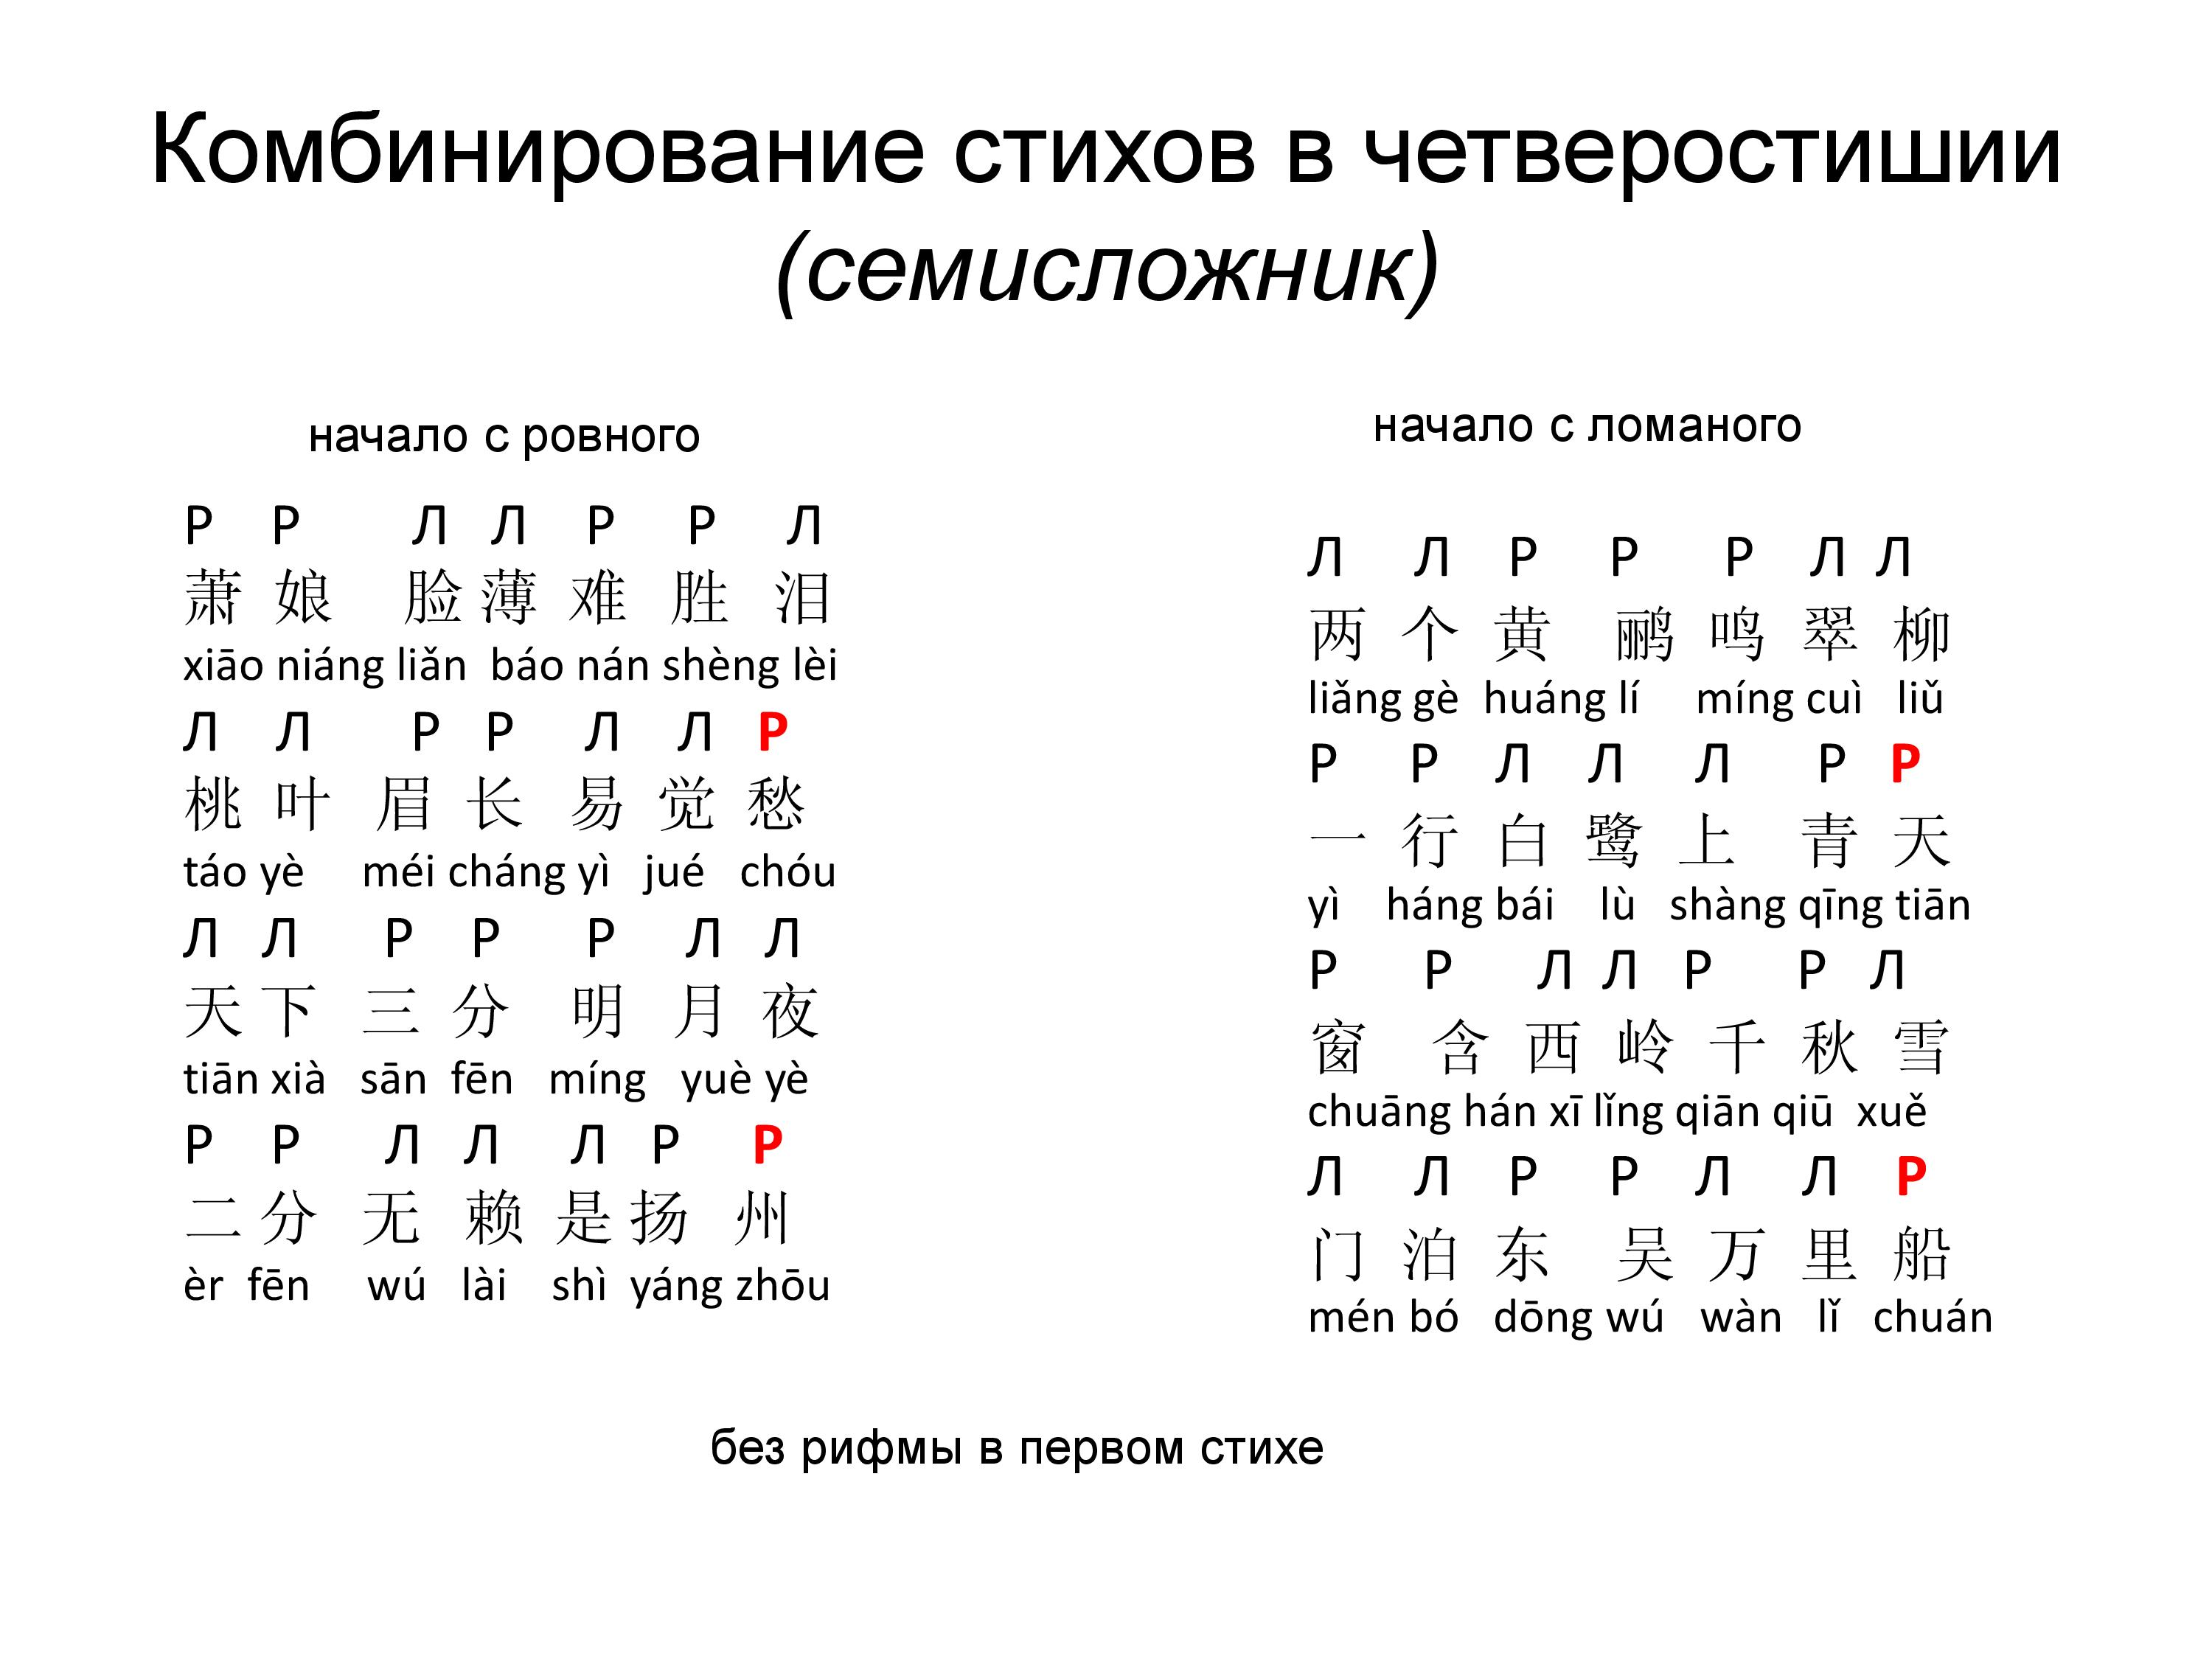
\includegraphics[width=0.8\textwidth]{cn.png}
\end{center}
\end{frame}

%------------------------------------------------

\subsection{Тоническая система}\label{sec:ton}

\begin{frame}
\frametitle{Если ритм~задаётся соизмеримым числом ударных слогов}

\begin{Parallel}{170pt}{}
\ParallelLText{
Ж\'{и}л"=был п\'{о}п,\\
Толок\'{о}нный л\'{о}б.\\
Пош\'{е}л п\'{о}п по~баз\'{а}ру\\
Посмотр\'{е}ть кой"=как\'{о}го тов\'{а}ру.\\
Навстр\'{е}чу ем\'{у} Балд\'{а}\\
Ид\'{е}т, сам не~зн\'{а}я куд\'{а}.\\
<<Что, б\'{а}тька, так~р\'{а}но подн\'{я}лся?\\
Чег\'{о} т\'{ы} взыск\'{а}лся?>>\\
П\'{о}п ем\'{у} в отв\'{е}т:\\
<<Н\'{у}жен мн\'{е} раб\'{о}тник:\\
П\'{о}вар, к\'{о}нюх и пл\'{о}тник.\\
А гд\'{е} найт\'{и} мне так\'{о}го\\
Служ\'{и}теля не сл\'{и}шком дорог\'{о}го?>>
}
\ParallelRText{Ак2 \'{—} $\smile$ \'{—}\\Ак2 $\smile$ $\smile$ \'{—} $\smile$ \'{—}\\Ак3 $\smile$ \'{—} \'{—} $\smile$ $\smile$ \'{—} $\smile$\\Ак3 $\smile$ $\smile$ \'{—} $\smile$ $\smile$ \'{—} $\smile$ \'{—} $\smile$\\Ак3 $\smile$ \'{—} $\smile$ $\smile$ \'{—} $\smile$ \'{—}\\Ак3 $\smile$ \'{—} $\smile$ $\smile$ \'{—} $\smile$ $\smile$ \'{—}\\Ак3 $\smile$ \'{—} $\smile$ $\smile$ \'{—} $\smile$ $\smile$ \'{—} $\smile$\\Ак3 $\smile$ \'{—} \'{—} $\smile$ \'{—} $\smile$\\Ак3 \'{—} $\smile$ \'{—} $\smile$ \'{—}\\Ак3 \'{—} $\smile$ \'{—} $\smile$ \'{—} $\smile$\\Ак3 \'{—} $\smile$ \'{—} $\smile$ $\smile$ \'{—} $\smile$\\Ак3 $\smile$ \'{—} $\smile$ \'{—} $\smile$ $\smile$ \'{—} $\smile$\\Ак3 {\small $\smile$ \'{—} $\smile$ $\smile$ $\smile$ \'{—} $\smile$ $\smile$ $\smile$ \'{—} $\smile$}}
\end{Parallel}
А.",С.",Пушкин, 1830

\end{frame}

%------------------------------------------------

\subsection{Силлабо-тоническая система}\label{sec:syl-ton}

%------------------------------------------------

\begin{frame}
\frametitle{Если ритм задаётся правильным чередованием ударных и~безударных слогов}
\begin{flushleft}
система стихосложения: силлабо"=тоническая
\end{flushleft}


\begin{Parallel}{160pt}{}
\ParallelLText{

Тр\'{и} д\u{е}в\'{и}ц\u{ы} п\`{о}д \u{о}кн\'{о}м\\
Пр\'{я}л\u{и} п\'{о}здн\u{о} в\`{е}ч\u{е}рк\'{о}м.\\
«К\'{а}б\u{ы} \'{я} б\u{ы}л\'{а} ц\u{а}р\'{и}ц\u{а}, "---\\
Г\`{о}в\u{о}р\'{и}т \u{о}дн\'{а} д\u{е}в\'{и}ц\u{а}, "---\\
Т\`{о} н\u{а} в\'{е}сь кр\u{е}щ\'{е}н\u{ы}й м\'{и}р\\
Пр\`{и}г\u{о}т\'{о}в\u{и}л\`{а} б я п\'{и}р».\\
«К\'{а}б\u{ы} \'{я} б\u{ы}л\'{а} ц\u{а}р\'{и}ц\u{а}, "---\\
Г\`{о}в\u{о}р\'{и}т \u{е}\'{е} с\u{е}стр\'{и}ц\u{а}, "---\\
Т\`{о} н\u{а} в\'{е}сь б\u{ы} м\'{и}р \u{о}дн\'{а}\\
Н\`{а}тк\u{а}л\'{а} я пол\u{о}тн\'{а}».

}
\ParallelRText{Х4м		\'{—} $\smile$ \'{—} $\smile$ — $\smile$ \'{—}\\Х4м		\'{—} $\smile$ \'{—} $\smile$ — $\smile$ \'{—}\\Х4ж		\'{—} $\smile$ \'{—} $\smile$ \'{—} $\smile$ \'{—} $\smile$\\Х4ж		— $\smile$ \'{—} $\smile$ \'{—} $\smile$ \'{—} $\smile$\\Х4м		— $\smile$ \'{—} $\smile$ \'{—} $\smile$ \'{—}\\Х4м		— $\smile$ \'{—} $\smile$ — $\smile$ \'{—}\\Х4ж		\'{—} $\smile$ \'{—} $\smile$ \'{—} $\smile$ \'{—} $\smile$\\Х4ж		— $\smile$ \'{—} $\smile$ \'{—} $\smile$ \'{—} $\smile$\\Х4м		— $\smile$ \'{—} $\smile$ \'{—} $\smile$ \'{—}\\Х4м		— $\smile$ \'{—} $\smile$ — $\smile$ \'{—}
}
\end{Parallel}
А.",С.",Пушкин, 1931

\end{frame}

% --------------------------------

\subsection{Силлабическая система}\label{sec:syl}

\begin{frame}
\frametitle{Если ритм задаётся соизмеримым 
количеством слогов}

система стихосложения: силлабическая

\textbf{С11ж}

\begin{verse}
Nel mezzo del cammin di nostra vita\\
mi ritrovai per una selva oscura\\
ché la diritta via era smarrita.

Ahi quanto a dir qual era è cosa dura\\
esta selva selvaggia e aspra e forte\\
che nel pensier rinova la paura!
\end{verse}
Dante Alighieri (1265\,--\,1321)

La Commedia, позже La Divina Commedia (1307\,--\,1321)

\end{frame}

%------------------------------------------------


\begin{frame}
\frametitle{Русский силлабический перевод Данте}
\textbf{С11ж}

\begin{verse}
На полдороге странствий нашей жизни\\
Я заблудился вдруг в лесу дремучем,\\
Попытки ж выйти вспять не удались мне

О, расскажу ли я о нем, могучем, \\
О диком лесе, лешей круговерти, \\
Где бедный ум мой был страхом измучен?
\end{verse}

\begin{flushright}
(пер. А.~А.~Илюшина)
\end{flushright}
\end{frame}



%------------------------------------------------

\begin{frame}
\frametitle{Стих как система компенсирующих 
речевых ограничений}

\begin{table}[]
\centering
\caption{Речь и стих}
\label{my-label}
\begin{tabular}{ll}
\hline
\multicolumn{1}{c}{Речь} & \multicolumn{1}{c}{Стих}          \\ \hline
Фиксированное ударение   & Свобода в~постановке ударения     \\
Разноместное ударение    & Ограничения в постановке ударения
\end{tabular}
\end{table}

Силлабика не ограничивает речь по~распределению ударных и~безударных слогов $\rightarrow$ дополнительные ограничения стиховой свободы $\rightarrow$ появляется ограничение на~словораздел в~стихе

\end{frame}

%------------------------------------------------
%
\begin{frame}
\frametitle{Ограничение на~словораздел в~стихе}

\begin{center}
Scène 1
\end{center}
Oreste
\begin{verse}
Oui, puisque je retrouve $\mid$ un ami si fidèle,\\
Ma fortune va prendre $\mid$ une face nouvelle;\\
Et déjà son courroux $\mid$ semble s'être adouci,\\
Depuis qu'elle a pris soin $\mid$ de nous rejoindre ici.

Безмерно счастлив я, $\mid$ что встретился с тобою!\\
Быть может, я теперь $\mid$ не так гоним судьбою?\\
Столь милостиво здесь $\mid$ она столкнула нас,\\
Что мнится — гнев ее $\mid$ теперь чуть-чуть угас.
\end{verse}
Жан Расин «Андромаха» 
1667

\end{frame}

%------------------------------------------------

\section{Русская силлабика}\label{sec:rusyl}

%------------------------------------------------

\begin{frame}
\frametitle{Когда в~России появилась поэзия?}
\begin{itemize}
\item в~народном творчестве "--- была всегда;
\item в~книжной литературе не~было оппозиции <<стихи\,--\,проза>>;
\item вместо этого была оппозиция <<то, что говорится\,--\,то, что поётся>>;
\item поэзия ли <<Слово о~полку Игореве>>? Да. Но~не~стихи;
\item идея нефольклорного стихотворства, облечённого в~социально значимые формы, была заимствована.
\end{itemize}

\end{frame}


\begin{frame}
\frametitle{Польская силлабика}
\textbf{С13ж}

\begin{verse}
Litwo! Ojczyzno moja! ty jesteś jak zdrowie.\\
Ile cię trzeba cenić, ten tylko się \alert{dowie},\\
\alert{Kto cię stracił}. Dziś piękność twą w całej ozdobie\\
Widzę i opisuję, bo tęsknię po tobie. 

Литва! О родина! Ты "--- как здоровье. Тот\\
Тебя воистину оценит и поймет,\\
Кто потерял тебя. Теперь живописую\\
Тебя во всей красе, затем, что я тоскую.

Отчизна милая, Литва! Ты как здоровье,\\
Тот дорожит тобой, как собственною кровью,\\
Кто потерял тебя. Истерзанный чужбиной,\\
Пою и плачу я лишь о тебе единой.
\end{verse}
Адам Мицкевич «Пан Тадеуш»
1832\,--\,1834

\end{frame}


\begin{frame}
\frametitle{Как заимствуются системы стихосложения}

\begin{itemize}
\item арабский \alert{аруз}: долгие и краткие слоги
\item метр мутак\={а}риб: $\smile$ — — 
\item известен благодаря персидской поэме <<Шах"=наме>> Фирдоуси, X~в.
\item в~тюркских языках нет долгих и~кратких слогов
\item допущение: считать закрытые слоги <<долгими>>, а~открытые <<краткими>> 
\end{itemize}

\lb{turk}{\gll bayat at{\i} birle s\"{o}z\"{u}g ba\c{s}lad{\i}m\\
\\$\smile$ --- ---$\mid\smile$ --- ---$\mid$ $\smile$ --- ---$\mid\smile$ ---
\trans С именем бога [свое] слово я начал\dots}
Юсуф Баласагунский <<Кутадгу билиг>> 

\end{frame}


\begin{frame}
\frametitle{Определения силлабики}

\begin{itemize}
\item «Силлаб\'{и}ческое стихослож\'{е}ние <\dots> "--- система стихосложения, осн. на~соизмеримости стихотв. строк по~количеству слогов (изосиллабизм)». \\
{\scriptsize Холшевников",В.",Е. Силлабическое стихосложение // Краткая литературная энциклопедия / Гл.~ред. А.",А.",Сурков. М.: Сов. энцикл., 1962\,--\,1978. Т.~6: Присказка\,--\,«Советская Россия», 1971. С.~819.}
\item «Изосиллаб\'{и}зм (греч. \textgreek{>isvosv\char212llaboc} "--- равносложный, от \textgreek{>'isvoc} "--- равный и \textgreek{svullab\char160} "--- слог) "--- одинаковое количество слогов в~отрезках речи. Используется и~в~прозе (см.~Изоколон) и~особенно в~поэзии, являясь, в~частности, основой силлабического стихосложения». \\
{\scriptsize Гаспаров",М.",Л. Изосиллабизм // Краткая литературная энциклопедия / Гл. ред. А.",А.",Сурков. М.: Сов. энцикл., 1962\,--\,1978. Т.~3: Иаков\,--\,Лакснесс, 1966. Стб.~74.}

\end{itemize}

\end{frame}

%------------------------------------------------

\begin{frame}
\frametitle{Силлабика и изосиллабизм}

«Нужно преодолеть широко распространенное заблуждение, согласно которому силлабический принцип отождествляется с~изосиллабизмом "--- равносложием строк в~пределах одного стихотворения. Изосиллабизм~же есть крайнее выражение, наиболее отчетливое воплощение силабического принципа, но~не~тождествен ему, поскольку силлабический принцип как~таковой требует не~выравнивания, а~всего лишь учета количества слогов в~строках».

{\scriptsize Илюшин",А.",А. Русское стихосложение. М.: Высш. шк., 2004. С.~17}

\end{frame}



%------------------------------------------------

\begin{frame}
\frametitle{Виршевая поэзия XVII века}
\begin{itemize}
\item Алексей Зюзин, конец XVI\,--\,начало XVII~в., русский чиновник и~дипломат времён Бориса Годунова и~последующего Смутного времени.
\item Михаил Игнатьевич Татищев (ум.~1609), русский государственный деятель и~дипломат, однофамилец известного экономиста и~историка XVIII~в. Василия Татищева (слово «тать» когда"=то имело широкое хождение).
\end{itemize}

{\scriptsize Виршевая поэзия: первая половина XVII века. / Сост., подгот. текстов, вступ. ст.~и~коммент. А.",А.",Илюшина, В.",К.",Былинина. М.: Советская Россия, 1989. 480~с.}
\end{frame}

%------------------------------------------------

\begin{frame}
\frametitle{Андрей Зюзин <<Послание Стефану Матвеевичу>>}

\begin{verse}
Великое убо светило на~тверди небесней тогда пресветле сияет и~вся твар уясняет,\\
егда лучезарнаго сияния темный облак не~закрывает.\\
Мысленое же солнце тогда паче преизобилует славою,\\
егда не~помрачено будет печалию многою.\\
Довлеет же, по апостолу, таковыя печаи лишатися, "---\\
от~нея~же вражде на~бога ражатися.\\
Печалование~же стяжати нам таково,\\
иже покаяние нераскаянново\\
спасение соделовает.\\
Которое~ж прежде возглаголю?\\
Свое~ли скорбное другу возвещу?\\
И~боюся, да~не~опечалую сим,\\
еже о~нас дружелюбнаго сердца,\\
или вопрошу о~настоящем благопребывании дружне,\\
<\dots>
\end{verse}

\end{frame}

%------------------------------------------------

\begin{frame}
\frametitle{Михаил Татищев <<Послание царю>>}

\begin{verse}
\textit{Великих превосочайших государей превосходящему властодержцу,\\
елико Уропии и Азии многих государств преславных самодержцу,\\
любителю и хранителю изрядну заповедей благословных\\
и доброопасному правителю закон православных.}

Которое таковому ныне принесу многое благодарение,\\
иже древних во благочестии сиятельных царей превосходит его милосердие,\\
им же российский скипетр преславно украшается,\\
государем великим пограничным выну страшем имянуется,\\
о нем же велелепная хвала в конца вселенныя истекает,\\
лава и богомудра и милостива всяка страна того нарицает\\
<\dots>
\end{verse}

\end{frame}

%------------------------------------------------

\begin{frame}
\frametitle{Симеон Полоцкий}
\begin{flushleft}
Симеон Полоцкий, 12~декабря 1629\,--\,25 августа 1680, самый известный русский стихотворец XVII~в. Самуил Гаврилович Петровский"=Ситнянович; Полоцкий "--- прозвище по~имени города. Автор поэтического сборника «Вертоград многоцветный» (1676\,--\,1680).
\end{flushleft}

\begin{figure}[ht]
  \begin{minipage}[ht]{0.49\linewidth}
    \center{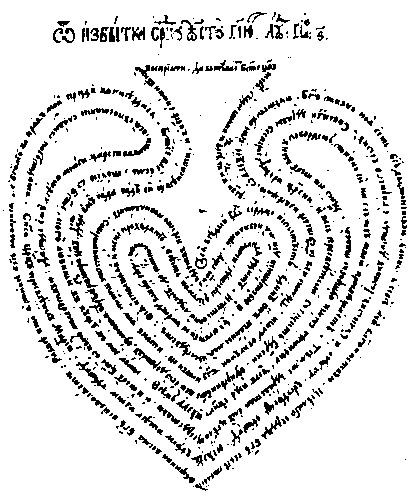
\includegraphics[width=0.4\linewidth]{Symeon_polotsky.png} \\ <<Благоприветствования>>}
  \end{minipage}
  \hfill
  \begin{minipage}[ht]{0.49\linewidth}
    \center{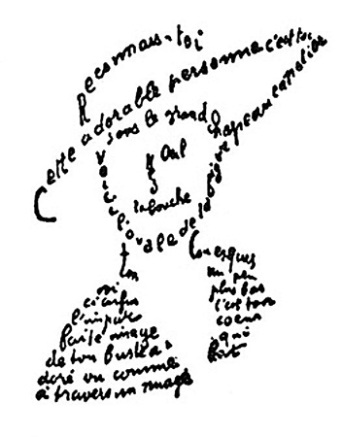
\includegraphics[width=0.4\linewidth]{apollinaire.jpg} \\ <<La femme au chapeau>>}
  \end{minipage}
  \caption{Визуальное тихотворение С.~Полоцкого и <<каллиграмма>> Г.~Аполлинера}
  \label{img:visual}  
\end{figure}

\end{frame}

%------------------------------------------------

\begin{frame}
\frametitle{Симеон Полоцкий}

\begin{center}
\textbf{Глас народа}
\end{center}

\begin{verse}
{\small Что наипаче от правды далеко бывает,\\
гласу народа мудрый муж то причитает.

Яко что-либо народ обыче хвалити,\\
то конечно достойно есть хулимо быти.

И что мыслить — суетно, а что поведает,\\
то никоея правды в себе заключает.

Еже гаждает — дело то весма благое,\\
а еже ублажает — то бохма есть злое.

В кратце, что-либо хвалит — то неправо в чести.\\
Мир сей непостоянный весь лежит в прелести.

Не веруй убо гласу общему народа\\
ищи в деле правды человеча рода. <\dots> 1678
}
\end{verse}

\end{frame}

%------------------------------------------------

\begin{frame}
\frametitle{Антиох Дмитриевич Кантемир}

\begin{flushleft}
10~сентября (21~сентября) 1708, Константинополь, по~другим данным Яссы\,--\,31~марта (11~апреля) 1744, Париж, Франция

Русский поэт"=сатирик и~дипломат, сторонник силлабической системы стихосложения. В~своих знаменитых сатирах (отнюдь не~смешных, что современному читателю непривычно) строил галереи образов, заслуживающих порицания.
\end{flushleft}


\end{frame}

%%------------------------------------------------

\begin{frame}
\frametitle{Антиох Кантемир}

\begin{center}
\textbf{Сатира I \\На хулящих учение {\small К уму своему}}
\end{center}

\textbf{С13ж}

\begin{verse}
Уме недозрелый, плод недолгой науки!\\
Покойся, не понуждай к перу мои руки:\\
Не писав летящи дни века проводити\\
Можно, и славу достать, хоть творцом не слыти.\\
Ведут к ней нетрудные в наш век пути многи,\\
На которых смелые не запнутся ноги;\\
Всех неприятнее тот, что босы проклали\\
Девять сестр. Многи на нем силу потеряли,\\
Не дошед; нужно на нем потеть и томиться,\\
\end{verse}

\end{frame}
%
%%------------------------------------------------
%
\begin{frame}
\frametitle{Сатира I. Продолжение}

\begin{verse}
И в тех трудах всяк тебя как мору чужится,\\
Смеется, гнушается. Кто над столом гнется,\\
Пяля на книгу глаза, больших не добьется\\
Палат, ни расцвеченна мраморами саду;\\
Овцу не прибавит он к отцовскому стаду.

«Расколы и ереси науки суть дети;\\
Больше врет, кому далось больше разумети;\\
Приходит в безбожие, кто над книгой тает, —\\
Критон с четками в руках ворчит и вздыхает,\\
И просит, свята душа, с горькими слезами\\
Смотреть, сколь семя наук вредно между нами\\
<...>
\end{verse}
1729

\end{frame}

%------------------------------------------------

\begin{frame}
\Huge{\centerline{продолжение следует}}
\end{frame}

\end{document}